\documentclass[12pt]{article}

\usepackage{prooftrees,amsmath,turnstile}

\usepackage{graphicx}
\graphicspath{ {./imgs/} }

\title{Symbolic Logic HW 2}
\author{Tyler Tracy}

\begin{document}

\maketitle

\section*{Solution to Problem 1}

\subsection*{Part (a)}

Argument: 
\begin{enumerate}
    \item $A \rightarrow [ (B \lor C) \rightarrow R]$
    \item $(R \lor S) \rightarrow T$
    \item $\therefore A \rightarrow (C \rightarrow T)$
\end{enumerate}

Truth tree: 

\begin{prooftree}
  {
    to prove={}
  }
  [A \rightarrow{} ((B \lor{} C) \rightarrow{} R), checked, just={(premise)}, name=pr
  [(R \lor{} S) \rightarrow{} T, checked, grouped, just={(premise)}
  [\lnot{} (A \rightarrow{} (C \rightarrow{} T)), checked, just={(conclusion)}
  [A, checked, just={3}
  [\lnot{} (C \rightarrow{} T), checked, just={3}
  [C, checked, grouped, just={5}
  [\lnot{} T, checked, just={5}
  [\lnot{} (R \lor{} S), just={2}, 
  [\lnot{} R, checked, just={8}
  [\lnot{} S, checked, just={8}
  [(B \lor{} C) \rightarrow{} R, just={1}
  [\lnot{} (B \lor{} C), just={11}
  [\lnot{} B, just={12}
  [\lnot{} C, just={12}, close={6}
  ]]]]
    [R, close={9}]
    ]]]]]
    [T, close={7}]
  ]]]]]
\end{prooftree}

This is a valid argument because the truth tree is closed.

\subsection*{Part (b)}

Argument:
\begin{enumerate}
    \item $\lnot A \rightarrow B$
    \item $C \rightarrow D$
    \item $\lnot B \lor D$
    \item $\therefore A \lor C$
\end{enumerate}

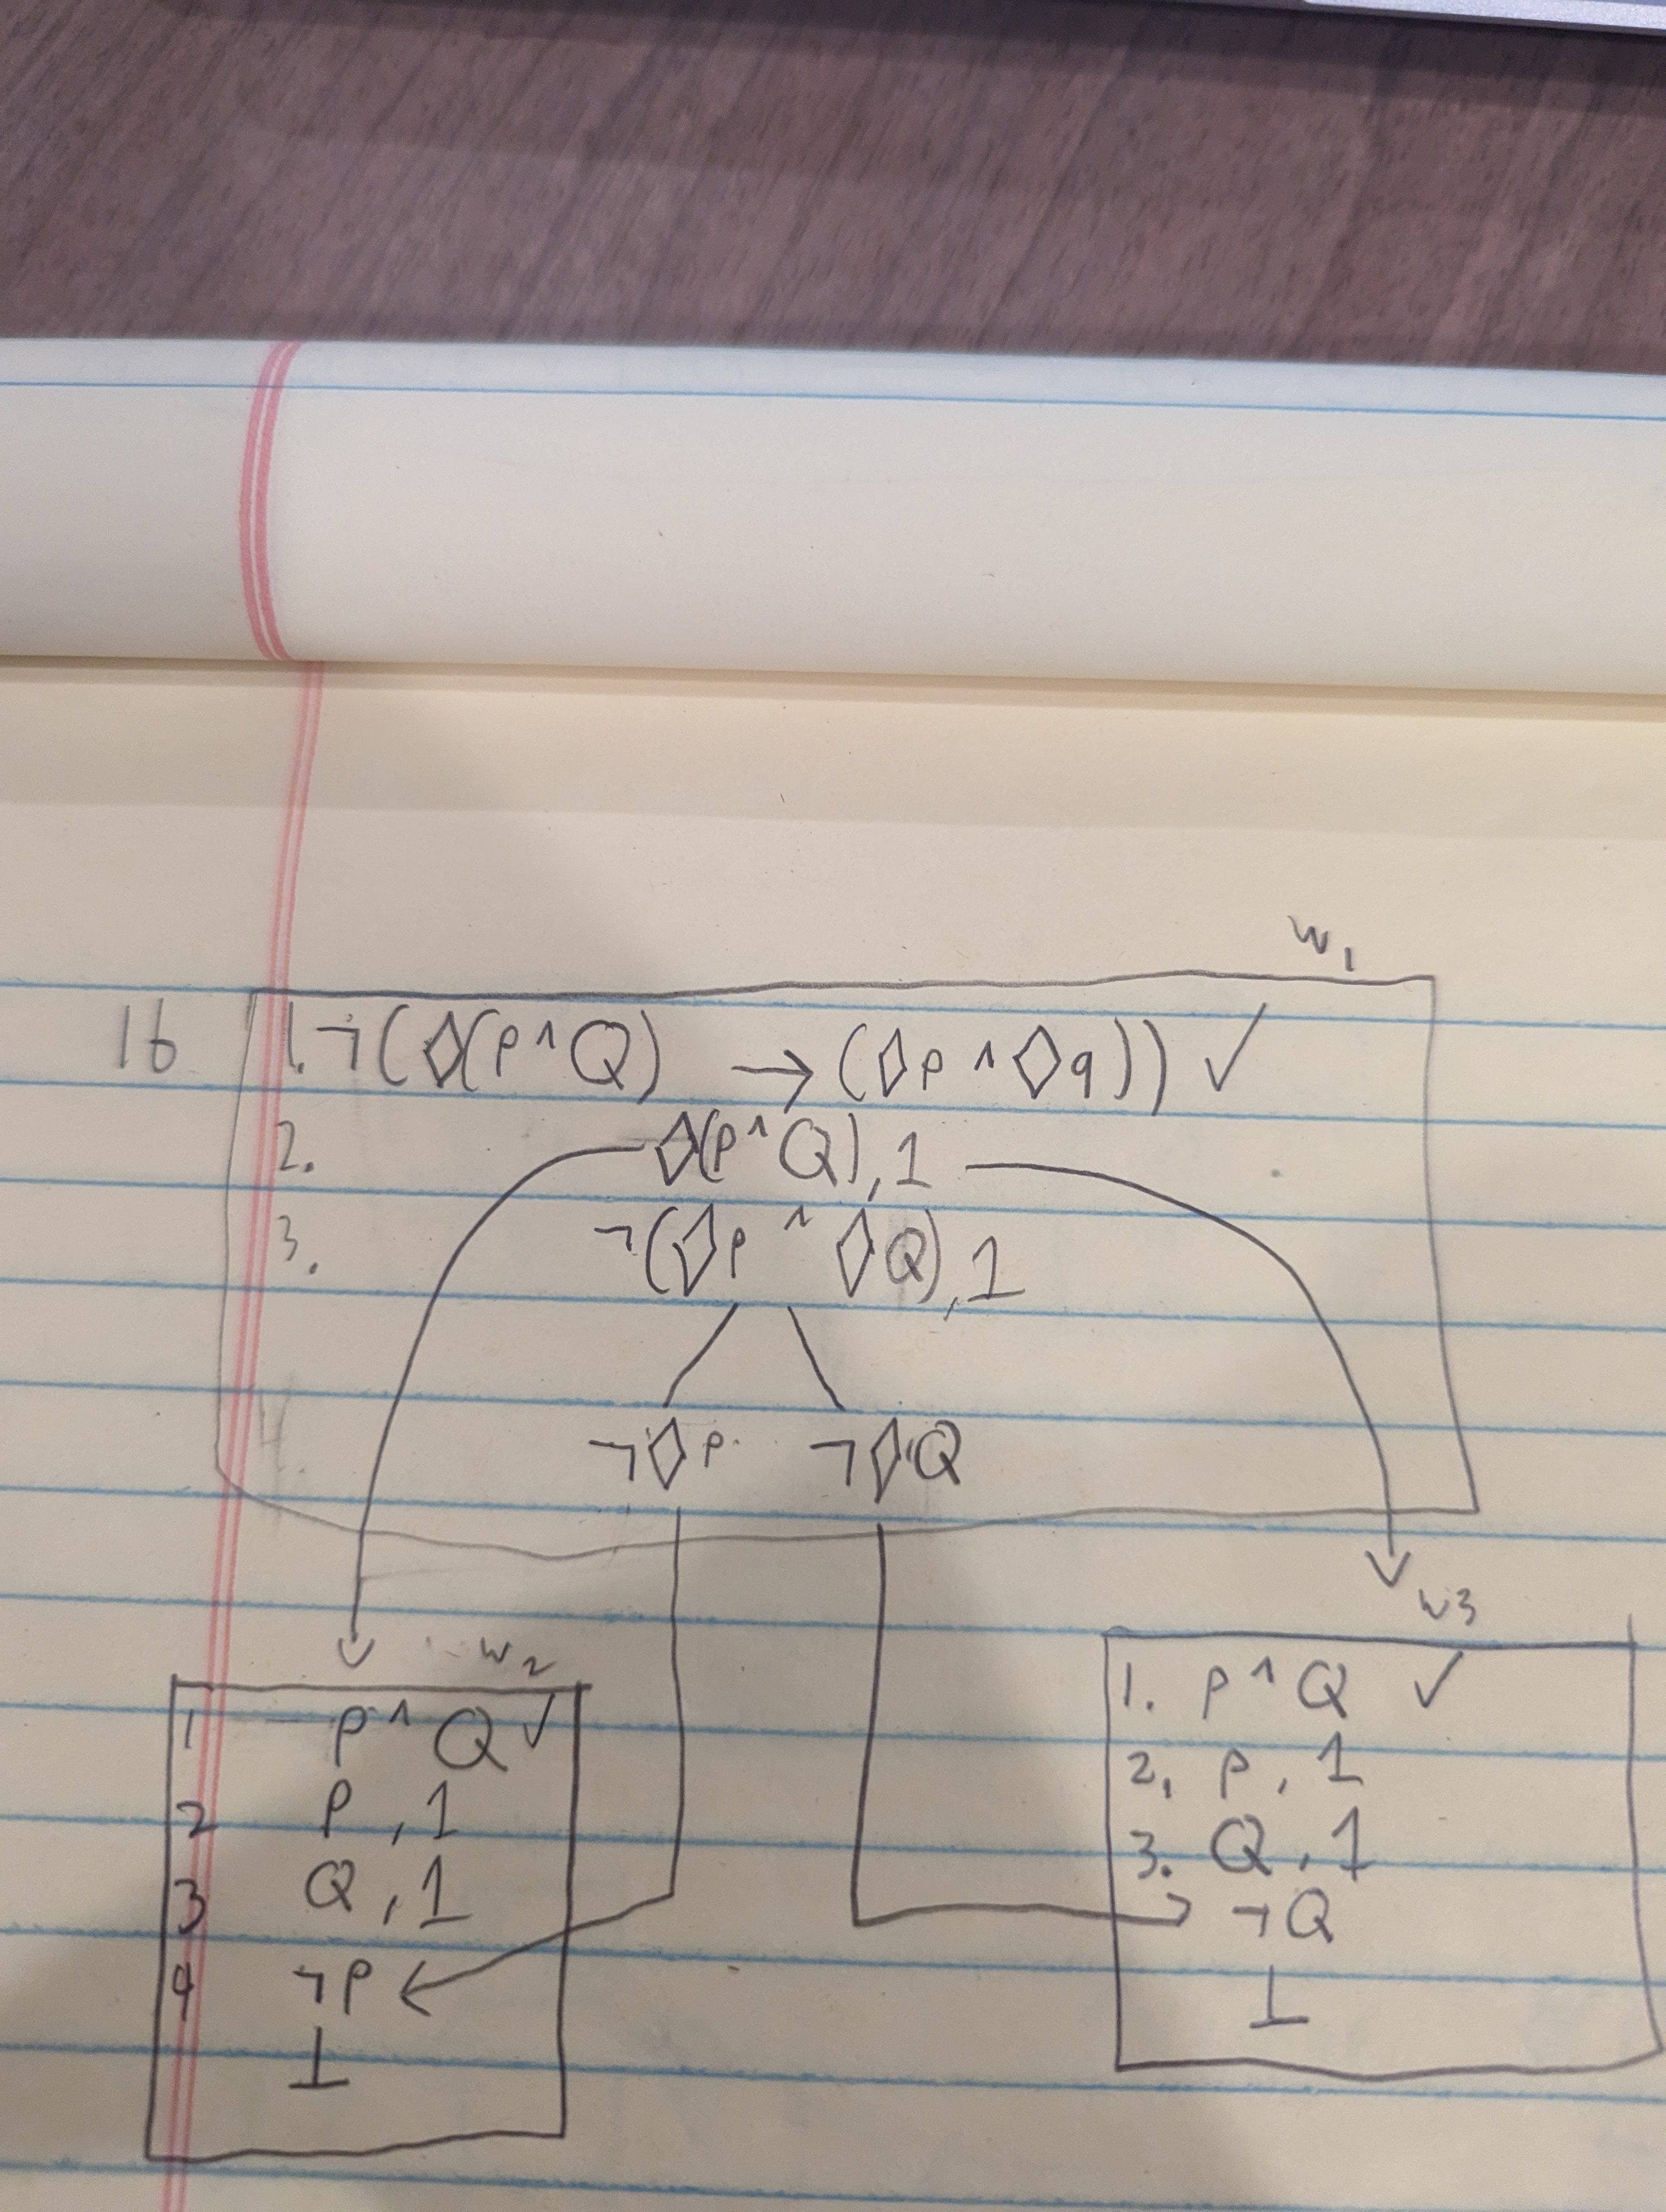
\includegraphics[width=\textwidth]{1b}

This argument is invalid. The following is a counterexample:

$\lnot A, \lnot B, \lnot C, D$

\begin{enumerate}
    \item $\lnot F \rightarrow T$, $T$ 
    \item $F \rightarrow T$, $T$
    \item $\lnot F \lor T$, $T$
    \item $F \lor F$, $F$
\end{enumerate}

The premises are true but the conclusion is false.

\subsection*{Part (c)}

Argument:
\begin{enumerate}
    \item $(Z \land M) \rightarrow (S \lor A)$
    \item $\lnot (Z \land S)$
    \item $\therefore (Z \land \lnot A) \rightarrow \lnot M$
\end{enumerate}

\includegraphics[width=\textwidth]{1c}

The argument is valid since the tree closes.

\section*{Problem 2}

To prove if something is a tautology, we negatate the sentence and show that the tree closes. 

\subsection*{Part (a)}

Sentence: $A \rightarrow (B \rightarrow A)$

\includegraphics[width=\textwidth]{2a}

This is a tautology since the tree closes.

\subsection*{Part (b)}

Sentence: $(B \leftrightarrow A) \leftrightarrow ((B \rightarrow A) \land (A \lor \lnot B))$

I'm going to quick simpify this by recognizing that $B \rightarrow A$ is logically equivalent to ($A \lor \lnot B$). So the sentence simpifies to the following

$(B \leftrightarrow A) \leftrightarrow (A \land \lnot B)$

\includegraphics[width=\textwidth]{2b}


This is not a tautology, $A, \lnot B$ is a counterexample. $(F \leftrightarrow T) \leftrightarrow (T \lor \lnot F)$ is false


\section*{Problem 3}

To prove logically equivalance, we can negate the biconditional between the two sentences and if the tree closes, they are equivalent. 

\subsection*{Part (a)}

Sentences: $A \rightarrow B$ and $B \rightarrow A$

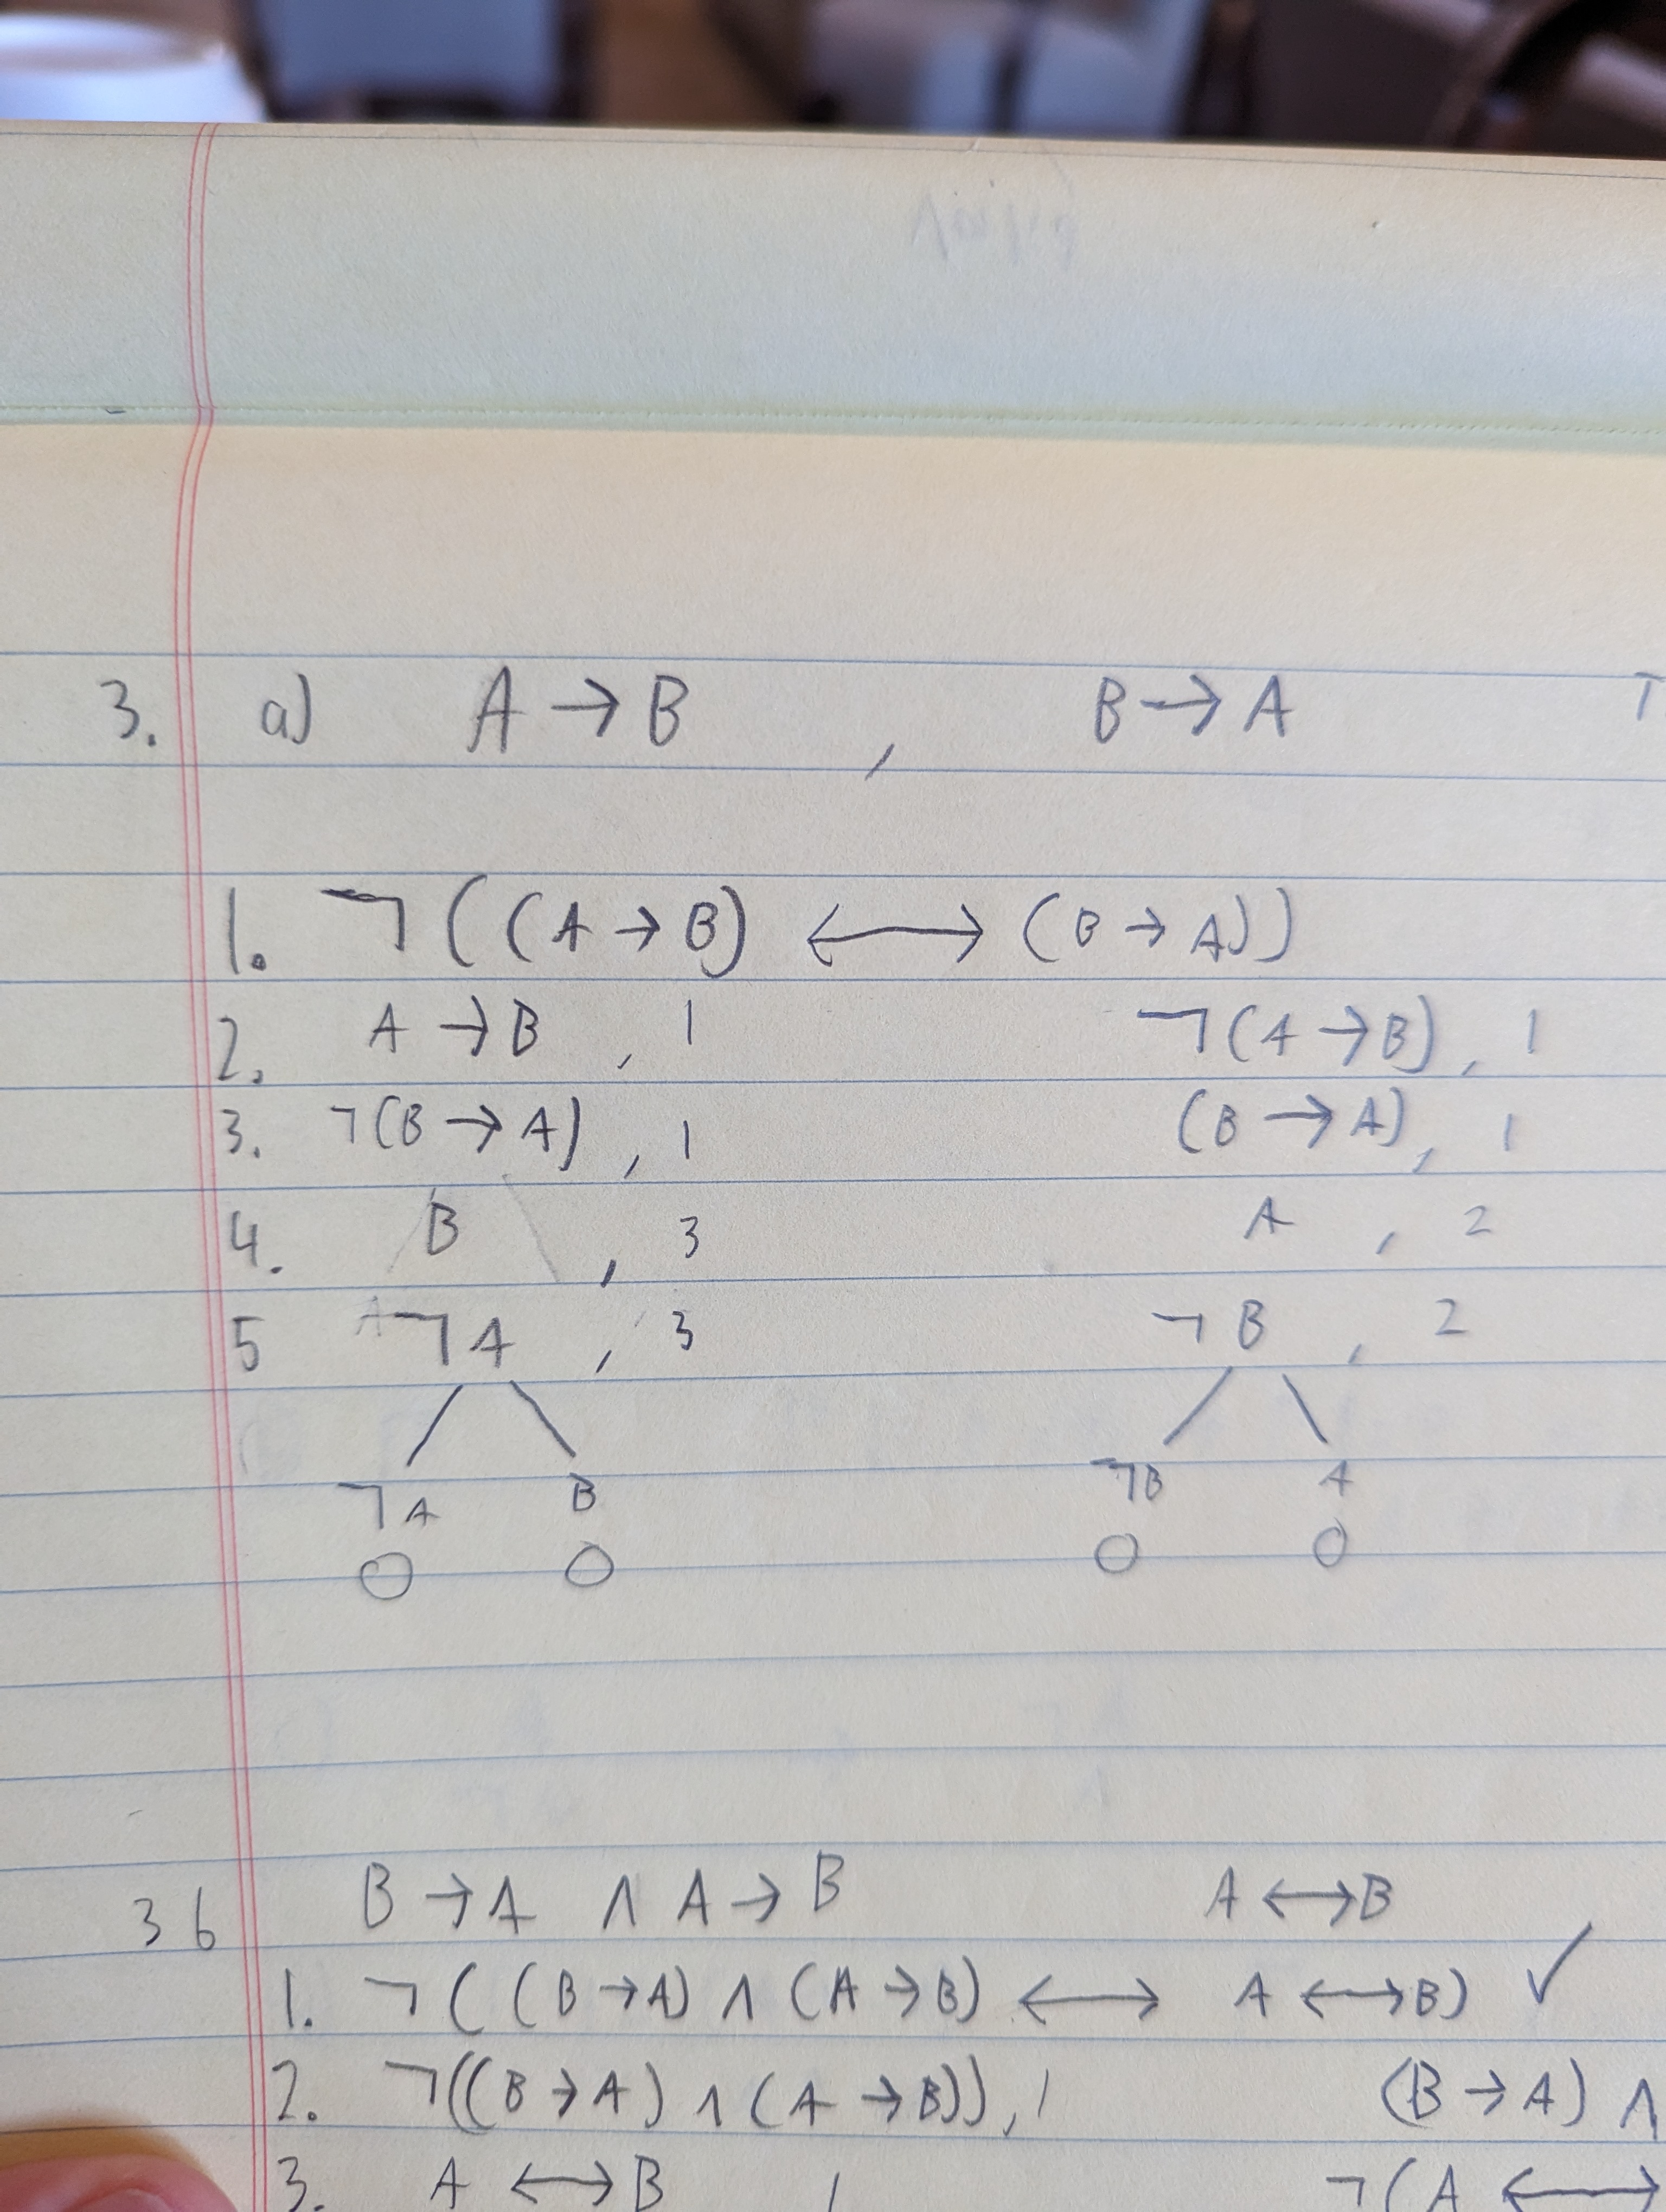
\includegraphics[width=\textwidth]{3a}

These two sentences are not logically equivalent. $A, \lnot B$ is a counterexample. $(F \rightarrow T) \leftrightarrow (T \rightarrow F)$ is false.


\subsection*{Part (b)}

Sentences: $(B \rightarrow A) \land (A \rightarrow B)$ and $A \leftrightarrow B$

\includegraphics[width=\textwidth]{3b}

These two sentences are logically equivalent since the tree closes. 

\section*{Problem 4}

\subsection*{Part (a)}

Claim: A sentence of form $p \lor q$ is a tautology if at least one of p and q is a tautology

\begin{enumerate}
    \item A sentence of form $p \lor q$ has truth table that always yeilds true, if at least one of p or q has a truth table that always yeilds true (by defintion of tautology)
    \item WLOG suppose p has a truth table that always yeilds true
    \item $p \lor q$ is always true since p is always true (by definition of logical or)
    \item This is true
\end{enumerate}

\subsection*{Part (b)}

Claim: For any set of sentence, $\Gamma$, if $\Gamma \vdash p \lor q$ then either $\Gamma \vdash p$ or $\Gamma \vdash q$.

This is false.

Suppose $\Gamma = \{p \lor q\}$. Then $\Gamma \vdash p \lor q$ but $\Gamma \nvdash p$ and $\Gamma \nvdash q$.


\subsection*{Part (c)}

Claim: If a set of sentences is inconsistent, then the set consisting of the negations of those sentences must be consistent. 

This is false.

Suppose $\Gamma = \{p, \lnot p\}$. Then $\Gamma$ is inconsistent but $\{\lnot p, p\}$ is also inconsistent.


\subsection*{Part (d)}

Claim: If the argument from the set of premises, $\Gamma$, to the conclusion ($A \land \lnot A$) is valid, then $\Gamma$ is inconsistent. 

\begin{itemize}
    \item If $\Gamma$ was consistent, then there would be a valid assignment of truth values that leds to all the sentences being true. 
    \item For a sentence to follow from $\Gamma$, it must be true in all of the truth assignments of $\Gamma$
    \item $A \land \lnot A$ is false in all truth assignments
    \item Therefore, $A \land \lnot A$ cannot follow from $\Gamma$
    \item We have a contradiction, so $\Gamma$ must be inconsistent
\end{itemize}

\section*{Problem 5}

Claim: $p$ and $q$ are logically equivalent if, and only if, $p \leftrightarrow q$ is a tautology. 



Prove if $p$ and $q$ are logically equivalent then $p \leftrightarrow q$ is a tautology.
\begin{itemize}
    \item $p$ and $q$ being loically equivalent means that they have the same truth tables
    \item Thus whenever $p$ is true, $q$ is true, and whenever $p$ is false, $q$ is false
    \item Thus the only two possible truth assignments for $p$ and $q$ are both true or both false
    \item $p \leftrightarrow q$ is true whenever $p$ and $q$ have the same truth assignment
    \item Thus $p \leftrightarrow q$ is true in all truth assignments
    \item Thus $p \leftrightarrow q$ is a tautology (by definition)
\end{itemize}

Prove if $p \leftrightarrow q$ is a tautology then $p$ and $q$ are logically equivalent.

\begin{itemize}
    \item $p$ and $q$ are a tautology if all truth assignments are true
    \item $p \leftrightarrow q$ is true whenever $p$ and $q$ have the same truth assignment
    \item $p$ and $q$ having the same truth assignment means that $p$ and $q$ are logically equivalent
\end{itemize}


\end{document}

